\section{Appendix}
\label{sec:appendix}

\subsection{Overview}
\noindent Our appendix includes the following:
\begin{itemize}
  \item \textbf{Section~\ref{sec:implementation}.} More details on model implementation and data setup.
  \item \textbf{Section~\ref{sec:additional_visuals}.} The chamfer distance graph for the truck category from OmniObject3D \cite{wu2023omniobject3d} and various visual results of our policy and the coverage baseline after 10 acquisitions on several objects and from various viewing angles. 
\end{itemize}

\subsection{Implementation Details}
\label{sec:implementation}

\noindent\textbf{Model Implementation.} We implement our model using Pytorch \cite{paszke2019pytorchimperativestylehighperformance} 
and carry out training using Pytorch Lightning \cite{Falcon_PyTorch_Lightning_2019}.
We leverage Pytorch3D\cite{ravi2020pytorch3d} to help create and render our point clouds. Our convolutional encoder has 4 layers and hidden dimension size of 256. Our rank MLP has 3 layers with a hidden dimension size of 256 and uses a CORAL \cite{coral2020} layer as its final layer so that a CORAL loss can be used during training. We use the open-source implementation of this loss and other necessary components provided by the authors on \href{https://github.com/Raschka-research-group/coral-pytorch}{GitHub}.

\noindent\textbf{Point Cloud Projection.} To project our point clouds to query views, we use the Pytorch3D\cite{ravi2020pytorch3d} PointsRasterizer with a points per-pixel setting of 1 and a fixed radius. Since the rasterizer uses a normalized coordinate system and our voxel down sampling leads to evenly spaced points, we find that this fixed radius size is sufficient. During the projection process for the point cloud we save a mapping from pixel to point allowing us to determine per-pixel feature vectors to construct a feature grid. We do all projection in batch.

\noindent\textbf{Model Training.} We train our model for 60 epochs using the AdamW\cite{loshchilov2019decoupledweightdecayregularization} optimizer and a cosine annealing\cite{loshchilov2017sgdrstochasticgradientdescent} learning rate scheduler. For our learning rate, we used 1e-3 and train for approximately 24 hours on four A6000 GPUs. During training time, we treat each set of next views for one specific object as a single batch. Batching by object means we only need to reconstruct one point cloud for an entire batch and can project it to all candidate views in one go, saving memory and computation.

\noindent\textbf{Evaluation Data Preparation.} The authors of GenNBV \cite{chen2024gennbv} resized the house objects from OmniObject3D \cite{wu2023omniobject3d} to better fit their problem context. The resized objects were made available by the authors on the project GitHub and we used them to calculate the exact scale factor applied to the original OmniObject3D \cite{wu2023omniobject3d} houses. We use this scale factor to bring our Chamfer Distance values computed on the unscaled objects into the correct scale for direct comparison. We also note that the point cloud for house 27 is missing and thus do not include it in evaluation since the correct scale factor cannot be calculated.

\begin{figure}[H]
  \centering
  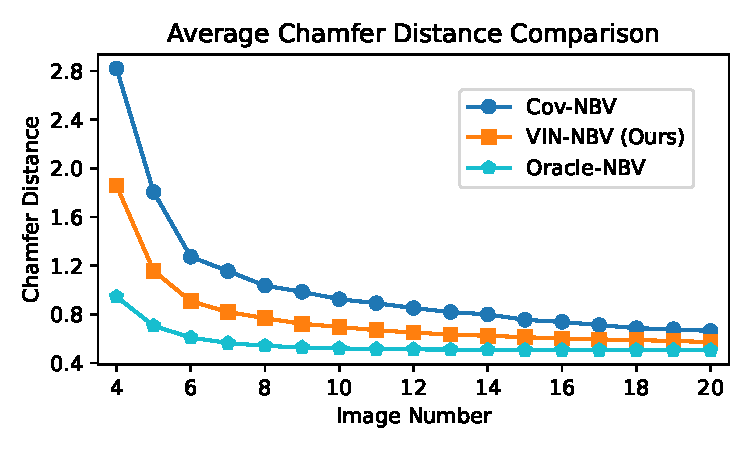
\includegraphics[width=0.96\columnwidth]{Figures/truck_combined_chamfer.pdf}
    \caption{Average Chamfer Distance across all truck objects from OmniObject3D \cite{wu2023omniobject3d} across each acquistion step.}
    \label{fig:truck_chamfer}
    \vspace{0.5em}
\end{figure}

\subsection{Additional Visualizations}
\label{sec:additional_visuals}

We include in the following pages visualizations of various objects after acquiring 10 captures in Fig.~\ref{fig:extra_visuals_p3}, Fig.~\ref{fig:extra_visuals_p2},
Fig.~\ref{fig:extra_visuals_p1}, and
Fig.~\ref{fig:extra_visuals_p4}. We compare the results of using VIN-NBV (ours) against a simple coverage baseline Cov-NBV. We show for each object two different perspectives to provide a comprehensive overview of the final reconstruction.

\clearpage
\begin{figure*}
  \centering
  \includegraphics[
  page=3,width=\textwidth,
  trim=10mm 12mm 10mm 12mm,clip,
  ]{Figures/extra_visuals.pdf}
  \vspace{-2.5em}
  \caption{
    Comparison of VIN-NBV and Cov-NBV after 10 acquisitions on motorcycles and houses from OmniObject3D\cite{wu2023omniobject3d}.
  }
  \label{fig:extra_visuals_p3}
\end{figure*}

\clearpage
\begin{figure*}
  \centering
  \includegraphics[
  page=2,width=\textwidth,
  trim=10mm 12mm 10mm 12mm,clip,
  ]{Figures/extra_visuals.pdf}
  \vspace{-2em}
  \caption{
    Comparison of VIN-NBV and Cov-NBV after 10 acquisitions on animals, house, and motorcycles from OmniObject3D\cite{wu2023omniobject3d}.
  }
  \label{fig:extra_visuals_p2}
\end{figure*}

\clearpage
\begin{figure*}
  \centering
  \includegraphics[
  page=1,width=\textwidth,
  trim=10mm 12mm 10mm 12mm,clip,
  ]{Figures/extra_visuals.pdf}
  \vspace{-2em}
  \caption{
    Comparison of VIN-NBV and Cov-NBV after 10 acquisitions on dinosaurs and animals from OmniObject3D\cite{wu2023omniobject3d}.
    }
  \label{fig:extra_visuals_p1}
\end{figure*}

\clearpage
\begin{figure*}
  \centering
  \includegraphics[
  page=4,width=\textwidth,
  trim=10mm 12mm 10mm 12mm,clip,
  ]{Figures/extra_visuals.pdf}
  \vspace{-20em}
  \caption{
    Comparison of VIN-NBV and Cov-NBV after 10 acquisitions on motorcycles and houses from OmniObject3D\cite{wu2023omniobject3d}.
  }
  \label{fig:extra_visuals_p4}
\end{figure*}
